\section*{Results}\linenumbers
\subsection*{Effects of sex, physiological state, and circadian timing on larval physiology} 
\noindent Behavioral experiments in insects have demonstrated the importance of circadian timing, starvation, and age \cite{Kaiser2008-me}. However, little is known about the effects of these variables on \textit{Ae. aegypti} larvae. To better understand the baseline characteristics of our study organism, we used machine vision to track individual \textit{Ae. aegypti} larvae in a custom arena (Fig 1A) and investigated the effects of nutritional state and sex on baseline larval behavior recorded before each experiment. For both fed and starved animals, female larvae were larger than males (fed larvae: n=120${\female}$, 128${\male}$, p<0.0001; starved larvae: n=79${\female}$, 89${\male}$, p=0.008, Fig S1A). Starved larvae were also smaller than fed animals for both females (p<0.0001) and males (p=0.015, Fig S1A). Because adult \textit{Ae. aegypti} exhibit crepuscular activity \cite{Christophers1960-xf}, we also investigated the effects of circadian timing on larval behavior. We found no effects of circadian timing on larval movement speed, time spent moving, or time spent next to arena walls - supporting previous findings that mosquito larvae, unlike adults, exhibit little behavioral variation during the day \cite{Van_Pletzen1981-qm,Clopton1979-in} (p=1, p=1, p=1, Fig S1B-D). 

\begin{figure}[t!]
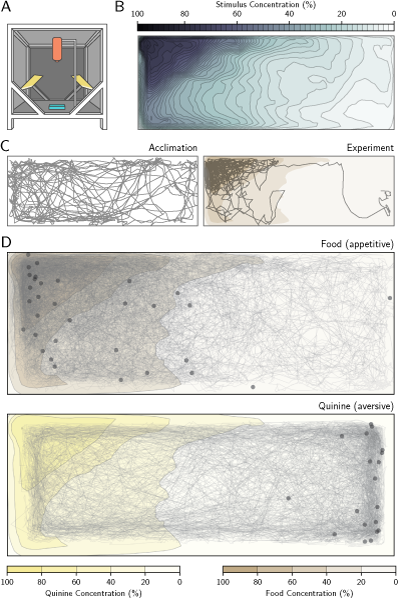
\includegraphics[width=\linewidth]{Figures/images/1.eps}
 \captionof{figure}{\textbf{Quantifying the chemosensory environment in naturalistic larval habitat sizes.} A: Diagram of experimental conditions, adapted from \cite{Bui2018-iq}, including a Basler Scout Machine Vision GigE camera (orange), infrared lighting (yellow) and a behavior arena (blue). B: Chemosensory diffusion map of the behavior arena at the end of the 15 minute experiment. C: Example of an individual larval trajectory during the 15 minute acclimation phase (left). Trajectory of same individual during the 15 minute experiment phase, responding to food added to the left side of the arena (right). D: Trajectory of all starved animals presented with food (top) or quinine (bottom). Although trajectories are shown aggregated into one image, all animals were tested individually. Scatter points show the position of each animal at the end of the experiment.  
 }
 \label{fig:fig1}
\end{figure}
\begin{figure*}[t!]
  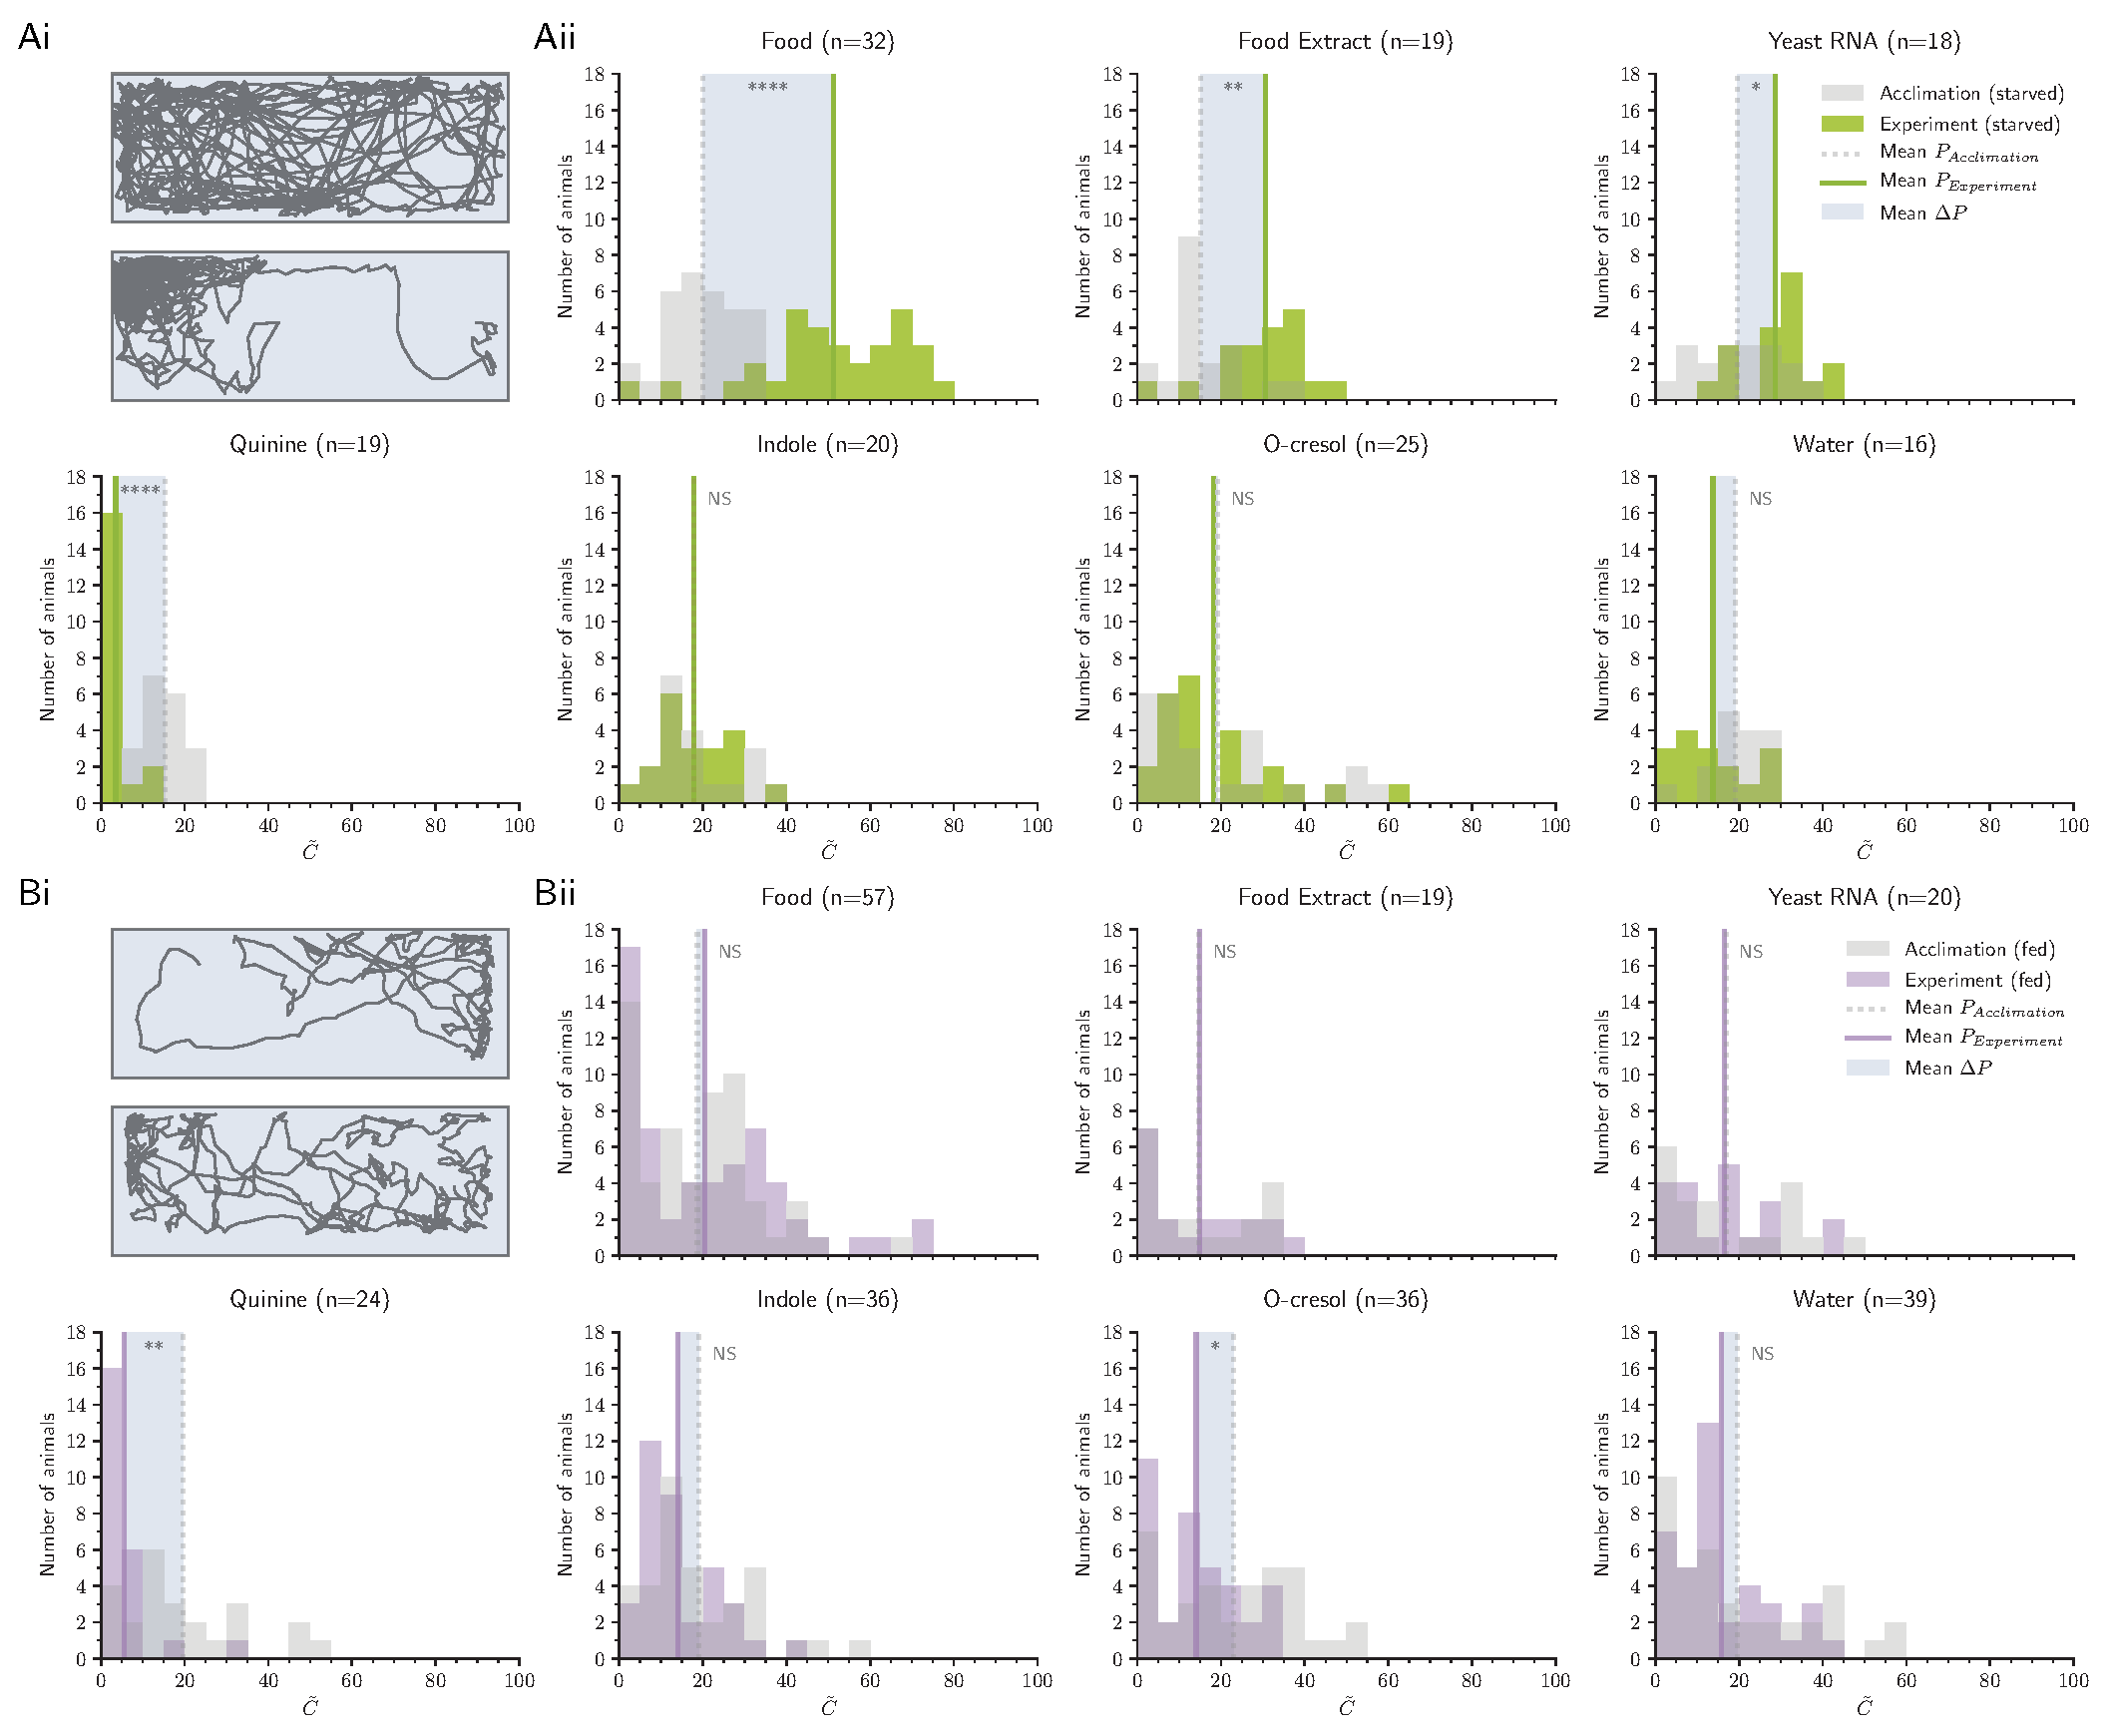
\includegraphics[width=\textwidth]{Figures/images/2.eps}
  \caption{\textbf{ Physiological feeding state affects larval attraction towards ecologically relevant odors.} Ai: Example trajectory of a starved larva during the acclimation (top) and the experiment phase (below), responding to food stimulus. Aii: Distribution of larvae during the acclimation phase (grey) and experiment phase (green), mean concentration ${\tilde{C}}$. The shaded box visualizes the mean ${\Delta}$P. Note that due to the unequal distribution of high and low concentration areas in the behavior arena, animals naturally appear to distribute near lower concentrations when no stimulus is present. Bi: Example trajectory of a fed larva during the acclimation (top) and experiment phase (below), responding to food stimulus. Bii: Distribution of fed larval preference during the acclimation (grey) and experiment phase (purple). In Aii and Bii, asterisks denote the significance level of paired-sample Welch's t-tests comparing acclimation P and experiment P (NS: not significant). N values reported next to each stimulus describe the number of animals in the treatment.
 }
\end{figure*}
\begin{figure*}[t!]
\bgroup \small \def\arraystretch{1.2}
\begin{tabular}{ l||c|c|c|c||c } \hline
    & \multicolumn{4}{c||}{\textbf{Potential Chemosensory Search Strategies}} & \\
     &\textit{Anosmic} & 
   \textit{Chemotaxis} & 
    \textit{Klinokinesis} &
    \textit{Chemokinesis} & \textbf{Experiment Observations} \\
\hline \hline
    Stimulus preference ${\Delta P}$ & no & 
    \cellcolor{yes}yes  & \cellcolor{yes}yes  & 
    \cellcolor{yes}yes  &\cellcolor{expyes}yes (p<0.0001)\\ 
\hline
    Directional preference ${\Delta DP}$ & no  & 
    \cellcolor{yes}yes  & no  & 
    no  & no (p=${0.18}$) \\  
\hline
    ${\Delta}$ Concentration speed ${\Delta DS}$ &  no  & 
     no   &  no  & 
     no  & no (p=${1}$) \\ 
\hline
    Concentration speed ${\Delta CS}$ & no  & 
    no & no  & 
    \cellcolor{yes}yes  &\cellcolor{expyes}yes (p<0.0001) \\ 
\hline
    ${\Delta}$ Concentration turns ${\Delta DTI}$ &  no  & 
    \cellcolor{yes}yes   &  no  & 
     no & no (p=${1}$)\\ 
\hline
    Concentration turns ${\Delta CTI}$ &  no  & 
     no & \cellcolor{yes}yes  & 
     no &  no (p=${1}$) \\ 
\hline \end{tabular} \egroup
\caption*{\textbf{Table 1: Comparing larval exploration behavior to canonical animal search strategy models.} Four different chemosensory search strategies are listed (central columns) along with the expected observable behavior metrics for each strategy (left column). By comparing the experimental observations (right column) with the expected results, we determined that \textit{Ae. aegypti} larval chemosensory navigation is best explained by an chemokinesis search strategy model.
}
\end{figure*}
\begin{figure}[!p]
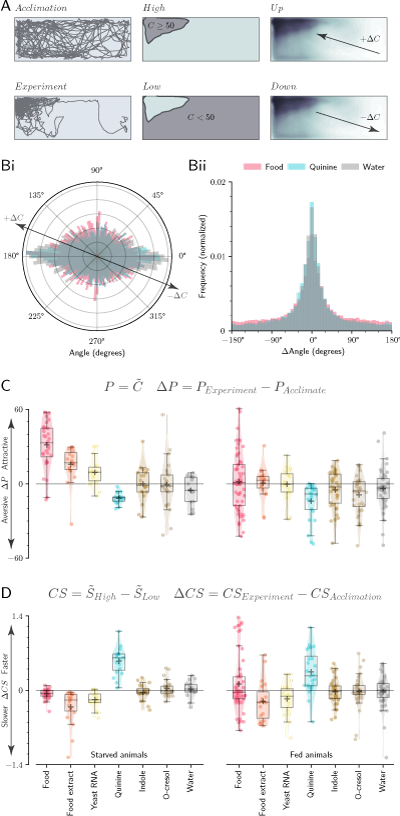
\includegraphics[width=\linewidth]{Figures/images/3.eps}
 \captionof{figure}{\textbf{ Larval exploration behavior is best explained by a chemokinesis search model.} A: Diagram of behavioral quantifications. Larvae were observed during a 15-minute acclimation period in clean water, followed by a 15-minute experiment in the presence of the stimulus. The arena was divided into an area of high (${\geq}$50${\%}$) and low concentration (<50${\%}$). Larvae could move in a direction that increased local concentration (+${\Delta}$C) or decreased local concentration (-${\Delta}$C). Bi: Orientation of animals in the arena throughout the experiment. Larvae did not exhibit directional movement in response to appetitive or aversive stimuli. Note that larvae spend more time moving horizontally (0${\degree}$, 180${\degree}$) because the rectangular arena is longer in the horizontal direction. Bii: Larvae did not change frequency of turns (${\Delta}$angle) in response to appetitive or aversive stimuli. C: Box plots for the population median (${\pm}$ 1 quartile), population mean (+ marker) and mean response for each individual (dots) for larval preference (${\Delta}$P). A horizontal line at 0 represents no change in behavior following stimulus addition. D: As in C, except for stimulus-dependent changes in Concentration-dependent Speed (${\Delta}$CS).
 }
 \label{fig:fig1}
\end{figure}

\subsection*{Quantifying the chemosensory environment in naturalistic larval habitat sizes} 
\noindent Previous research has shown that other species of mosquito larvae detect many different chemosensory stimuli \cite{Xia2008-hw}. In \textit{Ae. aegypti} it is unclear what chemical signals, if any, larvae use to navigate their environment. Nevertheless, chemosensory cues may be essential in avoiding predation or foraging efficiently. Using our arena and machine vision methods, we investigated larval preference for six putatively attractive and aversive chemosensory cues. First, we experimentally verified the chemical diffusion in the arena and found that larval activity significantly influenced the distribution of stimuli within the arena (p<0.0001). We next created a chemical diffusion map for analyzing stimuli preference using only experiments containing larvae (Fig 1B, Fig S2A-D). For chemosensory stimuli, we used predicted attractive stimuli including a 0.5${\%}$ mixture of food (Hikari Tropic First Bites fish food) suspended in water, as well as food extract filtered through a 0.2${\mu}$m filter to remove solid particulates. Quinine was used as a putative aversive stimulus (a bitter tastant aversive to many insects including \textit{Drosophila melanogaster} and \textit{Apis mellifera} \cite{Rusch2017-nf,El-Keredy2012-ke}). We also tested indole and o-cresol, two microbial compounds that attract adult mosquitoes for oviposition \cite{Afify2015-fi}. Finally, we examined the larval response to microbial RNA. RNA is required for \textit{Ae. aegypti} larval survival \cite{Akov1962-gy}, and nucleic acids attract larvae of several other mosquito species \cite{Merritt1992-op}. Moreover, dissolved RNA is released at high levels (${\mu}$g/h/L) from growing populations of microbes in freshwater habitats \cite{Paul_JH_undated-lx}, and could provide valuable foraging information to omnivores such as \textit{Ae. aegypti}. By contrast, other isolated macronutrients such as salts, sugars, and amino acids elicit little to no attraction \cite{Merritt1992-op}. 

\subsection*{Physiological feeding state affects larval attraction towards ecologically relevant odors} 
\noindent For each of these seven stimuli, we compared the stimulus preference of larvae before and after stimulus addition (Fig 1C, Fig 2A). Preference was defined as the median concentration chosen by the larvae throughout the 15-minute experiment, normalized to behavior during the previous 15-minute acclimation phase. Starved larvae were attracted to food (n=32, p<0.0001) and spent significantly less time near the aversive cue quinine (n=19, p<0.0001). Food extract filtered through a 0.2${\mu}$m filter remained attractive (n=19, p=0.004), suggesting that larvae use small, waterborne chemical cues to forage. To further investigate these foraging cues, we next examined responses to microbial RNA, and found that RNA was significantly attractive (n=18, p=0.047). Addition of water - a negative control for mechanical disturbance - had no impact on larval positional preference (n=16, p=1). Although we expected indole and o-cresol, which are attractive to adult \textit{Ae. aegypti}, to elicit attraction from larvae, neither odorant elicited a change in behavior from the acclimation phase (indole: n=20, p=1; cresol: n=25, p=1). Indole tested at a higher concentration (10mM) also had no effect (n=19, p=0.28). Together, these results suggest that larvae and adults may not necessarily rely on similar cues to assess larval habitat quality. 

The physiological feeding state of an adult mosquito has a strong impact on subsequent behavioral preferences \cite{Takken2001-lr}, and recent work has shown that larvae also exhibit appetite-dependent behavioral modifications \cite{Kinney2014-wn}. We thus fed larvae ad libitum to fish food before testing their responses to each of the seven chemosensory cues (Fig 2B). Fed larvae showed no significant attraction to food (n=57, p=1), food extract (n=19, p=1), and RNA (n=20, p=1), supporting the prediction that microbial RNA functions as an attractant in the context of foraging. Fed larvae showed no defects in quinine-mediated aversion (n=24, p=0.003), demonstrating that the lack of response to foraging cues is not due to a global reduction in chemosensory behavior. Similar to starved larvae, fed animals showed no preference for the water control (n=39, p=1) or indole (100${\mu}$M n=36, p=0.87, 10mM n=17, p=1). Fed larvae exhibited significant aversion to o-cresol (n=36, p=0.024).

\subsection*{Larval exploration behavior is best explained by a chemokinesis search model} 
\noindent Next we investigated the behavioral mechanism by which \textit{Ae. aegypti} larvae locate sources of odor, since such information could provide insight into the chemosensory pathways that mediate the behaviors. We hypothesized that larval aggregation near attractive cues such as food is mediated by chemo-klino-taxis - a common form of directed motion observed in many animals and microbes \cite{Berg1972-ch,Roder2017-pb,Hussain2016-ct}. In chemo-klino-taxis (hereafter chemotaxis), animals exhibit directed motion with respect to a chemical gradient. Alternatively, larvae may exhibit chemo-ortho-kinesis (hereafter chemokinesis) - a process in which animals respond to local conditions by regulating speed rather than direction - or chemo-klino-kinesis (hereafter klinokinesis) - in which animals respond to local conditions by regulating turning frequency. Finally, larvae may be unable to detect chemosensory stimuli, and thus exhibit purely random behavior (hereafter anosmic).To differentiate between these strategies, we quantified six observable metrics used to characterize navigation behavior. By identifying which variables correlate with stimulus preference, we can infer which search strategy best explains larval behavior (Table 1). Surprisingly, we found no evidence for chemotaxis near attractive or aversive chemicals. Starved larvae did not exhibit kinematic changes characteristic of chemotaxis, such as directional preference (${\Delta}$DP, p=0.18, Fig S3A). Further, larvae could not increase odor localization efficiency above random chance: discovery time for all cues was comparable across treatments (${\Delta}$D, p=1, Fig S3B). Larvae also did not perform klinokinesis: Turning frequency was unaffected by either the instantaneous concentration the larvae experienced (${\Delta}$CTI, p=1, Fig S3C) or change in concentration (${\Delta}$DTI, p=1, Fig S3D). Instead, we found that larval activity was most consistent with chemokinesis. Larvae altered movement speed when experiencing high local stimuli conditions (${\Delta}$CS, p<0.0001, Fig 3D) but not when moving up or down the concentration map (${\Delta}$DS, p=1, Fig S3E). 

\begin{figure}[t!]
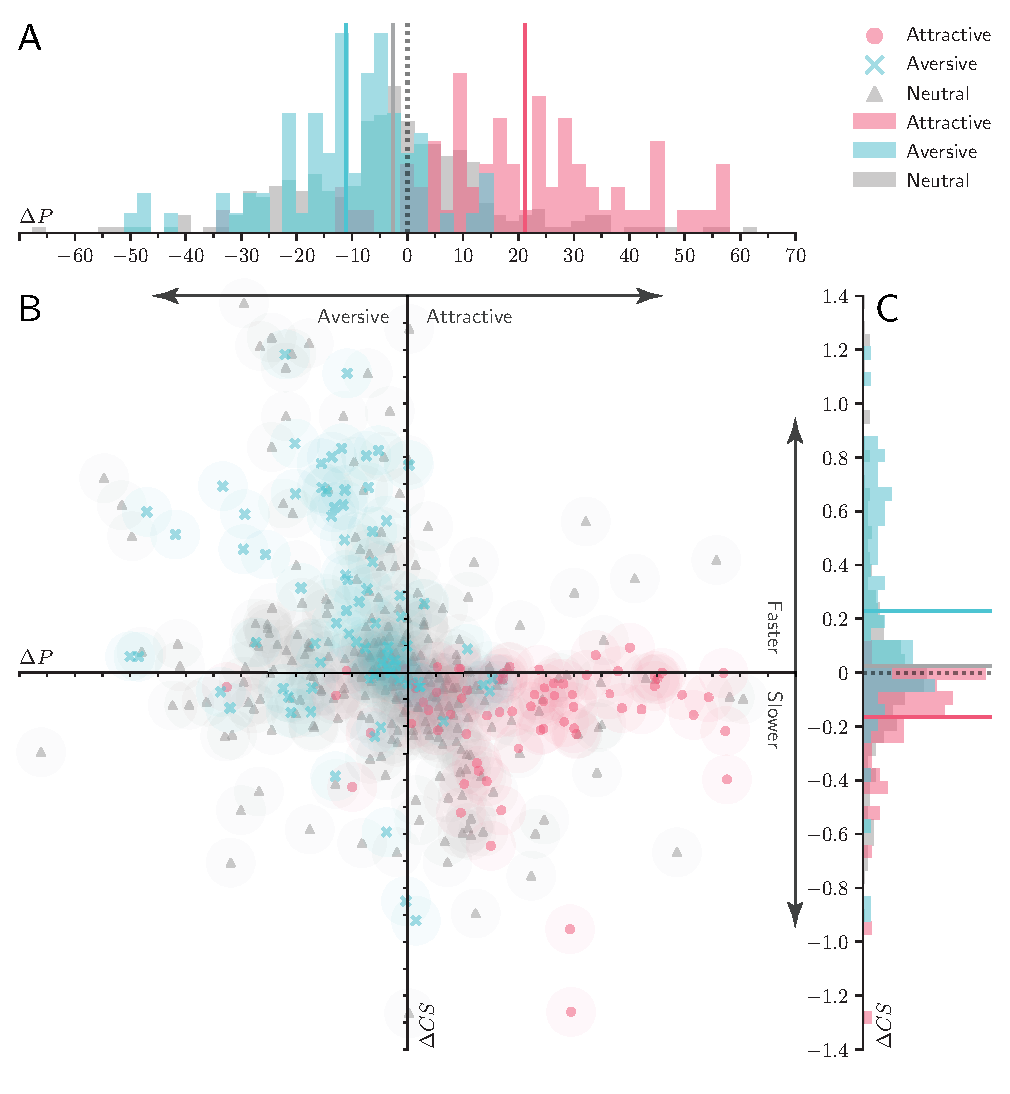
\includegraphics[width=\linewidth]{Figures/images/4.eps}
 \captionof{figure}{\textbf{Larval stimulus preference is correlated to concentration-dependent movement speed.} A: Larval preference (${\Delta}$P) significantly correlates with Concentration-dependent Speed (${\Delta}$CS). Results from all experiments are shown grouped into three categories: attractive (pink: food, food extract, and yeast RNA in starved larvae), aversive (blue: quinine), and neutral (grey: water, indole, o-cresol in fed and starved larvae; food, food extract, and yeast RNA in fed larvae). B: Normalized frequency histograms of ${\Delta}$P. Mean response to aversive, neutral, and appetitive cues are visualized as solid vertical lines in the corresponding color. A dotted black line at zero indicates the expected outcome if the added stimulus had no effect on larval behavior. C: As in B, except for normalized frequency histograms of larval ${\Delta}$CS.
 }
 \label{fig:fig1}
\end{figure}

\subsection*{Chemokinesis is superior to chemotaxis for avoiding repellents in realistic larval environments}
\noindent Our results were particularly surprising considering that many insects use chemotaxis rather than chemokinesis to navigate \cite{Gomez-Marin2011-tn}. Could chemokinesis be unusually advantageous in microhabitats, such as those utilized by mosquitoes in urban environments? We developed four data-driven models to simulate larval activity using chemokinesis, klinokinesis, an anosmic random walk, or chemotaxis. In these data-driven models, larval speed and turn angle was determined at each time step from a bootstrap resampling of empirical data from all larval trajectories in clean water (n=248 larvae during the acclimation phase, fed ad libitum. n=445,925 trajectory data points). This extensive empirical dataset allowed us to investigate the success of each search strategy while retaining the characteristics of authentic larval behavior. In addition, we created an exponential regression model to simulate diffusion properties observed in our experimental arena (p<0.0001, Fig S2E). Using these data-driven representations of larval speed, larval turning rate, and chemical diffusion in naturalistic larval habitats, we compared the success of each simulated search strategy in two separate challenges: a foraging task measuring time elapsed before finding a food source, and a repellent-avoidance task measuring the proportion of time spent in high-repellent environments. The success of each search strategy was explored across a range of common habitat sizes observed in urban environments \cite{Chan1971-sr} (Table 2). If larval chemokinesis is an adaptation to small urban microhabitats, we expect the chemokinesis search model to perform better than other strategies, and for this difference to be more apparent at smaller habitat sizes. Indeed, we found that chemokinesis was by far the best strategy in the repellent-avoidance task when avoiding potentially stressful environments (e.g. toxins, pollutants, or pesticides). Further, the difference between strategies was greatest at small habitat sizes (Fig 5A,B). 

\subsection*{Starved \textit{Aedes aegypti} optimize exploration behavior to increase the probability of finding food}
\noindent In contrast, chemokinesis was also the worst strategy in the foraging task, taking over an hour to find the simulated food source (Fig 5C,D). However, our data-driven models resampled empirical data collected from animals fed ad libitum. Many organisms change their speed or activity rate when starved \cite{De_Jager2014-if}, and we predicted that starved \textit{Ae. aegypti} may also alter their exploration behavior to increase the probability of discovering food \cite{De_Jager2014-if}. Experimental observations showed evidence for starvation-mediated behavior changes - starved animals spent more time exploring (p<0.0001, Fig 6A) and spent less time near walls and corners (p<0.0001, Fig 6B). If these starvation-mediated behavioral changes are adaptative, we expect the data-driven chemokinesis model to perform much better at the foraging task when given empirical data from starved larvae. Thus we tested the success of each search model in the foraging task using bootstrap resampling of empirical data from starved animals (n=168 starved larvae during the acclimation phase, n=302,096 trajectory data points). The starved chemokinesis model discovered the food source almost an hour faster across all habitat sizes (Fig 6C), supporting our hypothesis that starvation-mediated changes in larval behavior increase the probability of finding food. 

Nevertheless, starved chemokinesis simulations still performed worse than all other strategies in the foraging task. This result, coupled with the runaway success of the chemokinesis model in the repellent-avoidance task, suggests that avoiding repellents may be particularly important for \textit{Ae. aegypti} larval fitness. If avoiding repellents is essential for \textit{Ae. aegypti}, any starvation-mediated behavioral adaptations may be constrained by the additional requirement of retaining successful repellent-avoidance behavior. If so, we would expect to see very little difference in repellent-avoidance success across simulations based on empirical data from fed or starved larvae. Our results supported these predictions: Although starved simulations performed slightly worse compared to fed simulations, the difference was small: starved simulations only spent an average of 1${\%}$ more time near the repellent (Fig S4C). 

\begin{figure}[t!]
\bgroup \small \def\arraystretch{1.2}
\begin{tabular}{ l|l|l|l } 
    & \textbf{Radius} & 
    \textbf{Frequency} & \textbf{Examples}  \\
\hline \hline
    \textbf{i} & <5cm & 27.8${\%}$ of habitats & Ant traps \\ 
\hline
   \textbf{ii} & 5-9cm & 9.7${\%}$ of habitats & Tin cans, bottles \\ 
\hline
   \textbf{iii} & 9-17cm & 32.3${\%}$ of habitats & Jars, bowls, vases \\ 
\hline
    \textbf{iv} & 17-20cm & 3.1${\%}$ of habitats & Plates, pails \\ 
\hline \end{tabular} \egroup
\caption*{\textbf{Table 2: Ecologically realistic habitat sizes analyzed through computational modeling.} A range of habitat sizes were selected from a literature search of realistic habitat sizes for \textit{Ae. aegypti} larvae (\cite{Chan1971-sr} and references therein). 
}
\end{figure}
\begin{figure}[t!]
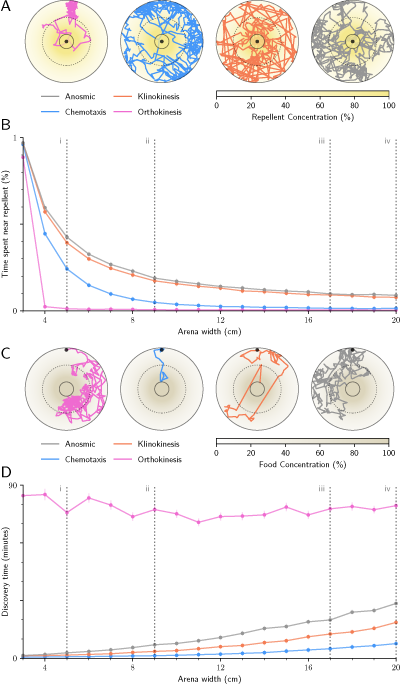
\includegraphics[width=\linewidth]{Figures/images/5.eps}
 \captionof{figure}{\textbf{Chemokinesis is superior to chemotaxis for avoiding repellents in realistic larval environments.} A: Sample trajectories for the repellent-avoidance task. B: Success of each search strategy in the repellent-avoidance task (mean ${\pm}$ standard error). C: Sample trajectories for the foraging task. (A,C): Dotted lines mark 50${\%}$ concentration. Foraging trajectories begin at the top of the 6cm-diameter arena, and repellent-avoidance task trajectories at the arena center (black dot). Starting point was randomized in actual analyses. D: Success of simulated search strategies in the foraging task. (B,D): Dashed grey lines correspond to ecologically relevant habitat sizes described in Table 2.}
 \label{fig:fig1}
\end{figure}